%!TEX root = ../template.tex
%%%%%%%%%%%%%%%%%%%%%%%%%%%%%%%%%%%%%%%%%%%%%%%%%%%%%%%%%%%%%%%%%%%%
%% chapter4.tex
%% NOVA thesis document file
%%
%% Chapter with lots of dummy text
%%%%%%%%%%%%%%%%%%%%%%%%%%%%%%%%%%%%%%%%%%%%%%%%%%%%%%%%%%%%%%%%%%%%

\typeout{NT FILE chapter4.tex}%

\chapter{Implementation}
\label{cha:implementation}

In this chapter, we present the implementation of our system.
We begin by offering an overview of system's architecture,
before delving into the implementation of each module in depth.

\section{Architecture} % (fold)
\label{sec:architecture}


The system was built using a modular approach;
each module is entirely self-contained, making it simple to expand or replace system functionality.
The system architecture is split into two distinct areas: the runtime, and the pipeline.
The runtime architecture comprises all essential components to the system liveness,
whereas the pipeline architecture covers all components needed during the system's provisioning and development.

\subsection{Runtime Architecture} % (fold)
\label{sec:runtime_architecture}

The runtime environment is supported by Kubernetes,
a simplified configuration with three microservices is depicted in Figure ~\ref{fig:runtime},
in this example, we have one micro-service that has undergone three major API changes the accounts micro-service, and
two micro-services that rely on it, the inventory micro-service that was updated to account for the changes, and the shipping micro-service which is two versions behind.

In Kubernetes a microservice is internally accessible through the Service abstraction;
a Service defines a policy for accessing a logical set of Pods via a load balancer with a
unique IP address that can be discovered thorough an environment variable, or an DNS name.

The containers of a pod are selected in services policies by attributing names to their exposed ports and assigning the same name on the target port of the service policy.
In adapter containers we expose one port for each of the supported versions and name each port with the respective version.

We define one service for each major version that is still being consumed, as shown in Figure ~\ref{fig:runtime},
older versions are supported by the adapter, while the most up to date version is directly supported by the microservice app.
A consumer accesses a producer app via the service that haves the same version as the one that it's expected in the static code.

When a microservice app is upgraded via a rolling update \footnote{A rolling update gradually replaces old replicas with new replicas},
the services never become unavailable, they point either to the adapter containers or the application containers, depending on whether the affected pods finished the upgrade process.

The only novel module introduced in the runtime environment is the proxy adapter;
the forthcoming modules are either developer tools or are invoked on stages of the DevOps pipeline.

\begin{figure}[htbp]
    \centering
    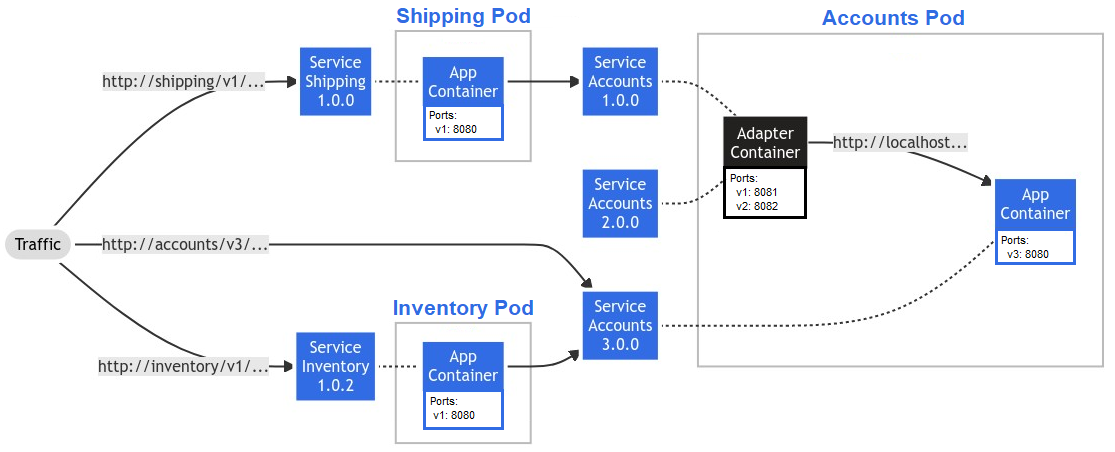
\includegraphics[height=2.4in]{runtime}
    \caption{Example of a runtime configuration}
    \label{fig:runtime}
\end{figure}

\subsection{DevOps Pipeline Architecture} % (fold)
\label{sec:devops_pipeline_architecture}

\begin{figure}[htbp]
    \centering
    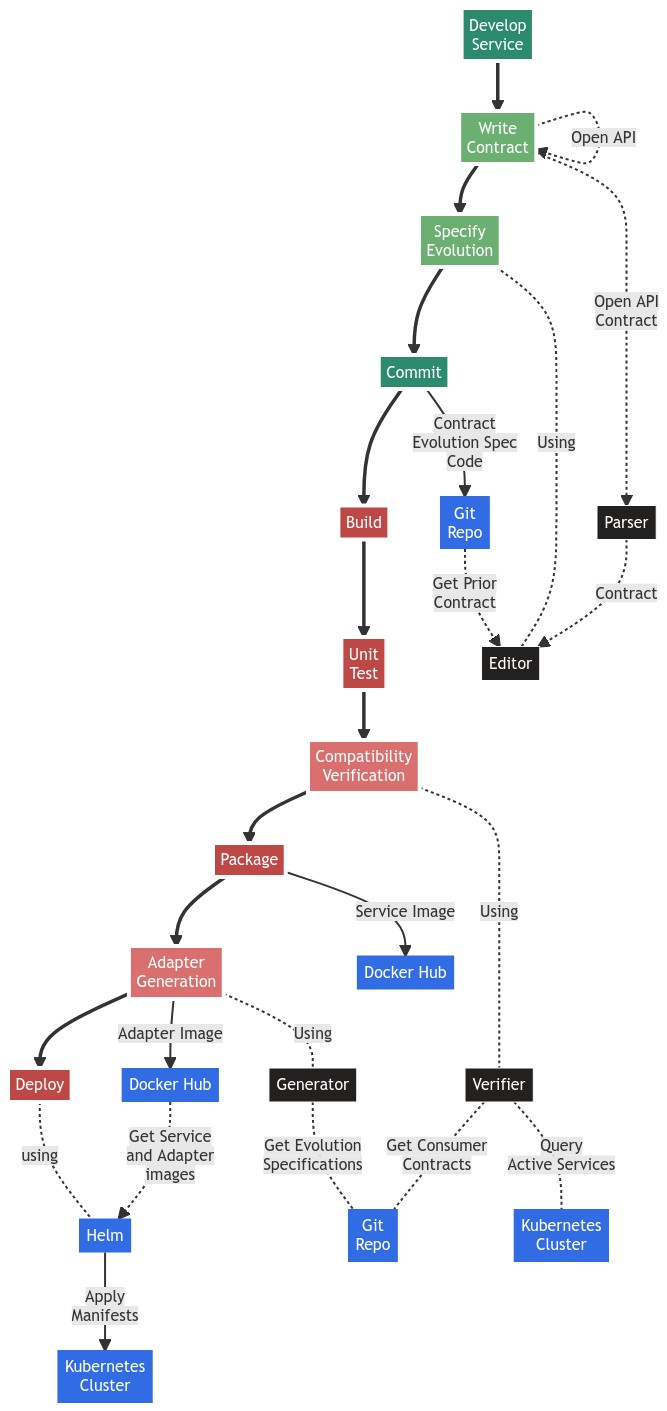
\includegraphics[height=9in]{DevOps}
    \caption{DevOps Pipeline}
    \label{fig:pipeline}
\end{figure}

\newpage

\section{Parser} % (fold)
\label{sec:parser}

\paragraph{Description}
\paragraph{Capabilities}
An HTTP contract contains the HTTP method, the
path, the parameter schema, and the location of parameters (path, query, header); the
proposed compatibility verification approaches supports all of these elements.
\paragraph{Limitations}
\paragraph{Dependencies}

\section{Editor} % (fold)
\label{sec:editor}

\paragraph{Description}
\paragraph{Capabilities}
\paragraph{Limitations}
\paragraph{Dependencies}

\section{Verifier} % (fold)
\label{sec:verifier}

\paragraph{Description}
\paragraph{Capabilities}
\paragraph{Limitations}
\paragraph{Dependencies}

\section{Generator} % (fold)
\label{sec:generator}

\paragraph{Description}
\paragraph{Capabilities}
\paragraph{Limitations}
\paragraph{Dependencies}

\section{Adapter} % (fold)
\label{sec:adapter}

\paragraph{Tuning}. The demo application image was built using Ubuntu 18.04.6 as a base image and consists of Spring-boot microservice with a Apache Tomcat/9.0.65 http server.
In order to prevent the JVM from resizing and reallocating the heap memory while Tomcat is trying to serve requests and
calling garbage collector frequently, the JVM has started with a higher heap memory maximum, and the initial heap memory
size was set to the same value as its maximum memory size.
The maximum number of threads for Tomcat was set to 2000, in order to support a higher load of requests.

\paragraph{Description}
\paragraph{Capabilities}
\paragraph{Limitations}
\paragraph{Dependencies}

\section{Registry} % (fold)
\label{sec:registry}

\paragraph{Description}
\paragraph{Capabilities}
\paragraph{Limitations}
\paragraph{Dependencies}
